% Fig. 2 of docs/nbcp/chapters/02-model-hamiltonian.tex: triangular lattice,
% nearest-neighbor vectors (one lattice step each) and Cartesian axes; the bond
% phases are given in the caption. Editable source; the PDF beside it
% (../bond-phases.pdf) is generated by examples/nbcp_research_export.py.
\documentclass[11pt,tikz,border=0pt]{standalone}
% Shared presentation settings for standalone TikZ figures; no scientific content.
% Keep the fonts and colors identical to ../../preamble.tex so that figure labels
% match the body text. Compile with XeLaTeX (see examples/nbcp_research_export.py).
\PassOptionsToPackage{dvipsnames,svgnames,x11names}{xcolor}
\usepackage{xcolor}
\usepackage{amsmath,amssymb}
\usepackage{unicode-math}
\defaultfontfeatures{Scale=MatchLowercase}
\defaultfontfeatures[\rmfamily]{Ligatures=TeX,Scale=1}
\setmainfont[BoldFont=texgyrepagella-bold.otf,ItalicFont=texgyrepagella-italic.otf,BoldItalicFont=texgyrepagella-bolditalic.otf]{texgyrepagella-regular.otf}
\setsansfont[BoldFont=texgyreheros-bold.otf,ItalicFont=texgyreheros-italic.otf]{texgyreheros-regular.otf}
\setmathfont{texgyrepagella-math.otf}
\setmathfont{texgyrepagella-math.otf}[version=bold,FakeBold=1.3]
\definecolor{NoteInk}{HTML}{24384A}
\definecolor{NoteAccent}{HTML}{126B78}
\definecolor{NoteMuted}{HTML}{63717B}
\definecolor{NotePale}{HTML}{F1F6F6}
\AtBeginDocument{\color{NoteInk}}


\begin{document}
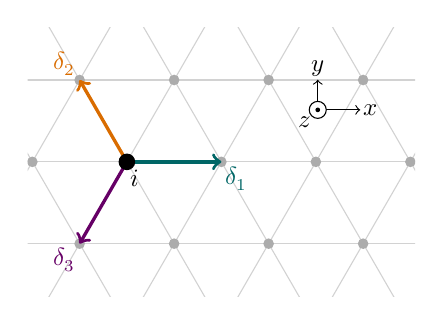
\begin{tikzpicture}[scale=1.2, font=\small]
  % Triangular Bravais lattice, adapted from the supplied source diagram.
  \begin{scope}
    \clip (-2.05,-1.42) rectangle (2.05,1.42);
    \foreach \m in {-4,...,4} {
      \foreach \n in {-3,...,3} {
        \coordinate (v) at ({\m-\n/2},{sqrt(3)*\n/2});
        \foreach \a in {0,60,120} {
          \draw[gray!35] (v)--++(\a:1);
        }
        \fill[gray!65] (v) circle (1.6pt);
      }
    }
  \end{scope}
  % Site i and its nearest-neighbor vectors: shifted one lattice step left (a lattice site).
  \begin{scope}[shift={(-1,0)}]
    \draw[->,very thick,teal!80!black] (0,0)--(0:1)
      node[below right,inner sep=1pt] {\(\boldsymbol\delta_1\)};
    \draw[->,very thick,orange!85!black] (0,0)--(120:1)
      node[above left,inner sep=1pt] {\(\boldsymbol\delta_2\)};
    \draw[->,very thick,violet!80!black] (0,0)--(240:1)
      node[below left,inner sep=1pt] {\(\boldsymbol\delta_3\)};
    \fill[black] (0,0) circle (2.5pt);
    \node[below right,inner sep=1pt] at (0,-0.05) {\(i\)};
  \end{scope}
  % Cartesian axes on the lattice (centered in the upper-right triangle, clear
  % of both the delta labels and the surrounding lattice lines).
  \begin{scope}[shift={(1.02,0.55)}]
    \draw[->] (0,0)--(0.45,0) node[right,inner sep=1pt] {\(x\)};
    \draw[->] (0,0)--(0,0.32) node[above,inner sep=1pt] {\(y\)};
    \draw[fill=white] (0,0) circle (0.09);
    \fill (0,0) circle (0.025);
    \node[below left,inner sep=1pt] at (-0.05,-0.03) {\(z\)};
  \end{scope}
\end{tikzpicture}
\end{document}
